\documentclass[10pt, a4papaer]{article}
\usepackage[utf8]{inputenc}
\usepackage{graphicx}
\usepackage[colorlinks,linkcolor=blue]{hyperref}
\usepackage{listings}
\usepackage{color}
\usepackage[hmargin=1.25in,right=1.25in,top=1in,bottom=1in]{geometry}
\usepackage{hyperref}

% listings setting
\definecolor{codegreen}{rgb}{0,0.6,0}
\definecolor{codegray}{rgb}{0.5,0.5,0.5}
\definecolor{codepurple}{rgb}{0.58,0,0.82}
\definecolor{backcolour}{rgb}{0.95,0.95,0.92}
 
\lstdefinestyle{mystyle}{
    backgroundcolor=\color{backcolour},   
    commentstyle=\color{codegreen},
    keywordstyle=\color{magenta},
    numberstyle=\tiny\color{codegray},
    stringstyle=\color{codepurple},
    basicstyle=\footnotesize,
    breakatwhitespace=false,         
    breaklines=true,                 
    captionpos=b,                    
    keepspaces=true,                 
    numbers=left,                    
    numbersep=5pt,                  
    showspaces=false,                
    showstringspaces=false,
    showtabs=false,                  
    tabsize=2,
    frame=single
}

\lstset{style=mystyle}

%%%%%%%%%%%%%%%%%%
\newcommand*{\titleGM}{\begingroup % Create the command for including the title page in the document
\hbox{ % Horizontal box
\hspace*{0.2\textwidth} % Whitespace to the left of the title page
\rule{1pt}{\textheight} % Vertical line
\hspace*{0.05\textwidth} % Whitespace between the vertical line and title page text
\parbox[b]{0.75\textwidth}{ % Paragraph box which restricts text to less than the width of the page

{\noindent\Huge\bfseries A brief Introduction to Git \\}\\[2\baselineskip] % Title
{\large \textit{Computer Version Class Assignment 01}}\\[4\baselineskip] % Tagline or further description
{\large \textsc{Zhu Guangyu\\[2\baselineskip]}} % Author name
{\large \textsc{20165953\\[3\baselineskip]}}
{\textsc{Github Repository: \href{https://github.com/z1ggy-o/assignment01.git}{assignment01\\[\baselineskip]}}}
{\textsc{\hyperlink{repo}{Repository Screenshot}}}

\vspace{0.5\textheight} % Whitespace between the title block and the publisher
}}
\pagestyle{empty}
\thispagestyle{empty}
\endgroup}

%%%%%%%%
% body
%%%%%%%%
\begin{document}

\titleGM %title page
\newpage

\tableofcontents
\newpage

%%%%%%%%%%%%%%%%%%%%%%%%%%%%%
% First section: What is Git?
%%%%%%%%%%%%%%%%%%%%%%%%%%%%%
\begin{section}{What Is Git?}

Git may be the most popular distributed version control system in the world.
It is created by Linus Torvalds for development of the Linux kernel. Git is
primarily used for source code management in software development, but it can
be used to for any set of files.

Next, let's briefly talk about the Version Control System and the features of
Git briefly.

%%%%%%%%%%%%%%%%%%%%%%%%%%%%%%%%%%%%
% subsection: version control system
%%%%%%%%%%%%%%%%%%%%%%%%%%%%%%%%%%%%
\begin{subsection}{Version Control System}

How do you manage your files? Do you do things like this when you try to modify
your files?
\begin{figure}[h]
    \centering
    
\includegraphics[width=0.8\textwidth]{images/old-file-management}
    \caption{"Old-fashion Version Control}
\end{figure}

With version control, you do not need to make duplicate files to avoid screw
your files up anymore. Version control system is a system that records changes
to files over time so that you can go back to the previous states. Also it
provides more features, such as comparing the differences between two versions
and collaborating with others.

\end{subsection}

%%%%%%%%%%%%%%%%%
% subsection: Git
%%%%%%%%%%%%%%%%%
\begin{subsection}{Git}

In general there are two types of version control systems, \textit{Centralized Version
Control Systems} and \textit{Distributed Version Control Systems}. Centralized
system has a client-server structure. All files are stored in a central server
and users just can access specific files which administrators allow them to.

Like we said before, Git is a \textit{distributed version control system}.
Instead of certain files, it fully mirror the repository from the server,
including history. This approach gives distributed system some advantages that
centralized system does not have. Such as users can work offline; if one server
dies, any client can restore it easily. Furthermore, we can have several remote
repositories working simultaneously within the same project.
    
\end{subsection}
\end{section}
\newpage

%%%%%%%%%%%%%%%%%%%%%%%%%%%%%%%
% Second section: How to use Git
%%%%%%%%%%%%%%%%%%%%%%%%%%%%%%%%
\begin{section}{How to Use Git}

At this part, let's talk about how to use git. I will just list some basic
operations to let you get into Git's world. If you want to know more,
\href{https://git-scm.com/book/en/v2}{\underline{Pro Git}} is a good book to read.
You can get it free online.

%%%%%%%%%%%%%%%%%%%%%%%%%%%%%%%%%%%%%%%%
% subsection: The basic construct of git
%%%%%%%%%%%%%%%%%%%%%%%%%%%%%%%%%%%%%%%%
\begin{subsection}{The Baic Construct of Git}

The files in git has three main states: committed, modified and staged:
\begin{itemize}
\item Modified means that you have changed something but have not put them into your database yet.
\item Staged means that you tell git which modified files you want to commit.
\item Committed files are files that stored in our local database
\end{itemize}

\begin{figure}[h]
    \centering
    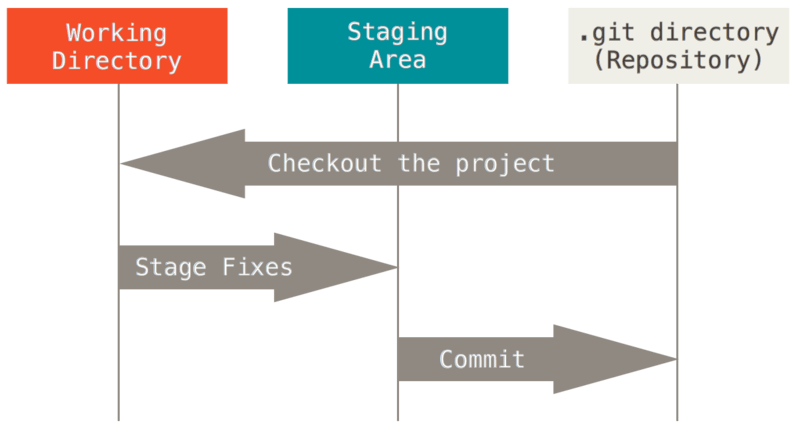
\includegraphics[width=0.8\textwidth]{images/git-stages}
    \caption{Git Stages}
\end{figure}

At the root directory of each git repository, you can find a hidden directory
called \textbf{.git}. This directory stores all the data for your project. When
you clone a repository from another computer, this is what you get. Delete .git,
you will lose everything.

Another thing I want to talk about is \textit{Branch}. One of the features of
git is that it supports non-linear developments well. Branching means you
diverge from the main line of development and to do some other works without
messing with main line. Git's branching operation's overhead is small. It does
not copy the files but use pointers to link your project snapshots together.
This approach makes creating branches fast and lightweight. That's why git
encourages people to do branch and merge often.

We will talk how to use branch later.
\newpage
\end{subsection}

%%%%%%%%%%%%%%%%%%%%%%%%%%%%%%%%%
% subsection: First time with git
%%%%%%%%%%%%%%%%%%%%%%%%%%%%%%%%%
\begin{subsection}{First Time with Git}

%%%%%%%%%%%%%%%%%%%%
% subsubsection: set name and email address
%%%%%%%%%%%%%%%%%%%%
\begin{subsubsection}{Set User Name and Email Address}

After the installation, the first thing to do is to set your name and email
address. This is important because Git uses this information to identify users.
Setting by command \verb+git config+:

\begin{lstlisting}
$ git config --global user.name "Your Name"
$ git config --global user.email "Your Email address"
\end{lstlisting}

Git's configuration files be stored in three different places and have different
scope. Use options below to `git config` to choose the scope you want. Each
level overrides the previous level:

\begin{lstlisting}
--system # apply to every user on the system
--global # apply to you, the user's repository
--local # apply to that single repository (default option)
\end{lstlisting}

There are many other variables we can modify. Check them once you got time.
\end{subsubsection}

%%%%%%%%%%%%%%%%%%%%
% subsubsection: First Repository %
%%%%%%%%%%%%%%%%%%%%
\begin{subsubsection}{First Repository}
\begin{paragraph}{Initial Repository\\}
    
Let's do our first commit together. Go to your project's directory, type 

\begin{lstlisting}
git init
\end{lstlisting}

This command will generate the \textbf{.git} subdirectory under the current directory.


At this point, nothing in the project is tracked yet. You have to tell Git
which files it should working on.

We can check the status of files through command \verb|git status|:
\begin{lstlisting}
$ git status

On branch master

No commits yet

nothing to commit (create/copy files and use "git add" to track)
\end{lstlisting}
\end{paragraph}

\begin{paragraph}{Track Files\\}
    
To track new files, use command \verb|git add <file>|.
This command will put files into the \textit{staging area}, both new files or
modified files. Only files in the staging area will be committed into the database.
Now, let's add some files:

\begin{lstlisting}
$ git add README.md assignment01.tex
$ git status
On branch master

No commits yet

Changes to be committed:
  (use "git rm --cached <file>..." to unstage)

	new file:   README.md
	new file:   assignment01.tex
\end{lstlisting}

We can find the two files are staged and will to into our next commit.
\end{paragraph}

\begin{paragraph}{Commit\\}
    
Now let's finish our first commit, just type \verb|git commit|.
Git will ask you to input the commit message:

\begin{lstlisting}

    # Please enter the commit message for your changes. Lines starting
  3 # with '#' will be ignored, and an empty message aborts the commit.
  4 #
  5 # On branch master
  6 #
  7 # Initial commit
  8 #
  9 # Changes to be committed:
 10 #   new file:   README.md
 11 #   new file:   assignment01.tex
 12 #
\end{lstlisting}

Writing meaningful commit message is very important, because the message is the
best way to learn about a change. Google "How to write a good git commit", you 
commit message, but well formed message helps a lot.\\
can find lots of articles talking about it. There is no standard way to write
\end{paragraph}

\begin{paragraph}{Check History\\}
    
Use \verb|git log| we can check the existing commit history:

\begin{lstlisting}
commit 7af35596163c980d0661faeef9a3eef1e67732be (HEAD -> master)
Author: Guangyu Zhu <guangyuzhu1129@gmail.com>
Date:   Mon Sep 17 22:04:38 2018 +0900

    Third commit

commit 38697bada55cf777d069613760f90a24dd09b792
Author: Guangyu Zhu <guangyuzhu1129@gmail.com>
Date:   Mon Sep 17 22:03:49 2018 +0900

    Second commit

commit b2e78948dde81c0ca5858e4f78d52a4b0676c368
Author: Guangyu Zhu <guangyuzhu1129@gmail.com>
Date:   Mon Sep 17 21:35:30 2018 +0900

    Initial the project.
\end{lstlisting}

There are hash values for each commit. Git use the hash values to identify
commits. By the way, this is a example of bad commit messages. You can get
nothing meaningful from above commit messages.

With these hash values we can go back to previous commit through command\\
\verb|git checkout <hash>|:

\begin{lstlisting}
$ git checkout b2e78948
Note: checking out 'b2e78948'.

You are in 'detached HEAD' state. You can look around, make experimental
changes and commit them, and you can discard any commits you make in this
state without impacting any branches by performing another checkout.

If you want to create a new branch to retain commits you create, you may
do so (now or later) by using -b with the checkout command again. Example:

  git checkout -b <new-branch-name>

HEAD is now at b2e7894... Initial the project.
\end{lstlisting}

To go back to the newest commit, type \verb|git checkout master|.

\end{paragraph}
\end{subsubsection}

\begin{subsubsection}{Delete and Ignore Files}

Sometimes you tracked the wrong files or you want to remove some tracked files.
Delete them from the directory may not working well, because you need to tell
git to stop tracking them. Use \verb|git rm <file>| will remove the file from git
and working directory.

To avoid tracking some files that we do not need, \textbf{.gitignore} comes out.
List patterns to match file names in \textbf{.gitignore}. Git will ignore all
the files that are listed in \textbf{.gitignore} file.Git use \textit{glob patterns}
that shells use. If you do not know which files need to be ignored. Do not worry,
\href{https://www.gitignore.io/}{\underline{gitignore.io}} can generate these
rules for you. The only thing you need to do is input the working environment.
\end{subsubsection}
\end{subsection}

%%%%%%%%%%%%%%%%%%%%%
% subsection: Branch
%%%%%%%%%%%%%%%%%%%%%
\begin{subsection}{Branch}
    
It's time for branch now. Like we said before, git use pointer to link snapshots(commits)
together. That means we can use pointer to switch between snapshots easily. Creating
a new branch just creates a new pointer for us to move around.

\begin{paragraph}{Create Branch\\}
To create a new branch, use command \verb|git branch <branch_name>|:

\begin{lstlisting}
$ git branch testing
$ git branch
* master
  testing
\end{lstlisting}

\verb|git branch| command without any option will show us current branches.
The branch with \textbf{*} before it is the branch that we are working on.

\end{paragraph}

\begin{paragraph}{Switch Between Branches\\}

Switch to other branch by \verb|git checkout <branch_name>| command. We 
use same command to check previous commits. Since they are just snapshots linked
together. No actual difference between the normal commits and branches:

\begin{lstlisting}
$ git check out testing
Switched to branch 'testing'
\end{lstlisting}

Now you can do anything you want with your files. There is no impact on the content
on the master branch.
\end{paragraph}

\begin{paragraph}{Merge\\}

Assuming that we want to develop some new features. Here is the example of
branch-merge workflow.

First we go back to master branch and create another branch to start development:

\begin{lstlisting}
$ git checkout master
Switched to branch 'master'
$ git branch -b new_feature
$ Switched to branch 'new_feature'
\end{lstlisting}

\verb|git checkout -b <branch>| will create a new branch then move on it automatically.

After the development, we merge the \verb|new_feature| branch back into 
\verb|master| branch to deploy the feature. We do this with the \verb|git merge|
command:

\begin{lstlisting}
Updating 7af3559..2628c91
Fast-forward
 README.md | 1 +
 1 file changed, 1 insertion(+)
$ git checkout master
$ git merge new_feature

$ git branch
* master
  new_feature
  testing
\end{lstlisting}

Because we no longer need \verb|new_feature| branch, we can delete it with
\verb|git branch -d <branch>|:

\begin{lstlisting}
$ git branch -d new_feature
Deleted branch new_feature (was 2628c91).
\end{lstlisting}
\end{paragraph}

\begin{paragraph}{Conflict\\}
Let's do it again. This time we merge testing branch into master:

\begin{lstlisting}
$ git merge testing
Auto-merging README.md
CONFLICT (content): Merge conflict in README.md
Automatic merge failed; fix conflicts and then commit the result.
\end{lstlisting}

This is time something new occurs:
\begin{lstlisting}
CONFLICT (content): Merge conflict in README.md
\end{lstlisting}

What is conflict? Sometimes we modified same file on different branch, when we
merge two branches together, git cannot know which one is the file that we want.
Thus, we have to resolve those conflicts manually. Check status first:

\begin{lstlisting}
$ git status
On branch master
You have unmerged paths.
    (fix conflicts and run "git commit")
    (use "git merge --abort" to abort the merge)

Unmerged paths:
    (use "git add <file>..." to mark resolution)

    both modified:   README.md

no changes added to commit (use "git add" and/or "git commit -a")
\end{lstlisting}

The message tells us both branches modified \verb|README.md| file.
Use editor open README.md:

\begin{lstlisting}
<<<<<<< HEAD
Made some modification on branch new_feature
=======
Do some modification in branch testing
>>>>>>> testing
\end{lstlisting}

The content between \verb|<<<<<<<| and \verb|>>>>>>>| is the conflict part.
Top block is the content in current branch(in our case is master). Above block
is the content from incoming branch.

After we resolve the conflicts, stage the conflict file then commit the change:

\begin{lstlisting}
$ git add README.md
$ git commit

$ git status
On branch master
nothing to commit, working tree clean
\end{lstlisting}

Finished the merge! In this context, we have tried some of the most basic and
most commonly used commands. Next part we will talk about Github and how to use
Github as our remote server.
\end{paragraph}

\end{subsection}
\end{section}
\newpage
%%%%%%%%%%%%%%%%
% Third section: Github
%%%%%%%%%%%%%%%%
\begin{section}{Collaborate Through Github}

Github is a web-based hosting service for version control using Git. It is
commonly used to host open-source software projects. Github may be the largest
host of source code in the world.

Once you sign up a account, you can use it free if you make your repository
public.

With Github this platform, we can talk about working with remotes now.

%%%%%%%%%%%%%%%%%%%
% subsection: Remote repository
%%%%%%%%%%%%%%%%%%%%
\begin{subsection}{Remote Repository}

First, let's create a repository on Github:

\begin{figure}[h]
    \centering
    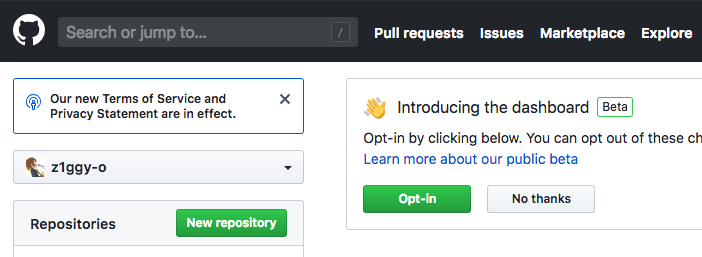
\includegraphics[width=0.8\textwidth]{images/create-repo}
    \caption{Create Repository}
\end{figure}

\begin{subsubsection}{Clone Repository}
    
Github will ask you to do the first commit to initial the repository. Usually
people will create a \textbf{README.md} file. After this, we can clone this 
repository to our computer.

\begin{figure}[h]
    \centering
    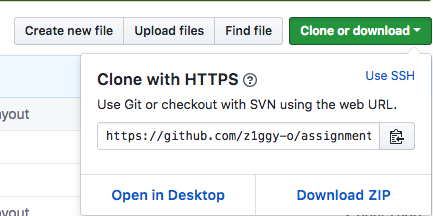
\includegraphics[width=0.5\textwidth]{images/clone-button}
    \caption{HTTPS URL}
\end{figure}

There are two ways to clone repositories: HTTPS or SSH. Github recommends users
to use HTTPS, so we will use HTTPS here.

Go to the directory where you want to download the repository. Use command
\verb|git clone <url>|:

\begin{lstlisting}
$ git clone https://github.com/z1ggy-o/assignment01.git
Cloning into 'assignment01'...
remote: Counting objects: 23, done.
remote: Compressing objects: 100% (18/18), done.
remote: Total 23 (delta 3), reused 19 (delta 2), pack-reused 0
Unpacking objects: 100% (23/23), done.
\end{lstlisting}

\verb|git clone| adds the \verb|origin| remote for us implicitly. We can use
command \verb|git remote| to show remote repositories:

\begin{lstlisting}
$ git remote -v
origin	https://github.com/z1ggy-o/assignment01.git (fetch)
origin	https://github.com/z1ggy-o/assignment01.git (push)
\end{lstlisting}

Here we can find the \verb|origin|. \verb|fetch| shows where we get data from
and \verb|push| shows where we upload our local files to.

\begin{paragraph}{Adding Remote Repositories\\}

We can bind our local repository with more than one remote repositories. Add remote
repositories by command \verb|git remote add <name> <url>|:

\begin{lstlisting}
$ git remote add assign-repo-2 https://github.com/z1ggy-o/another-assignment01.git
$ git remote -v
assign-repo-2	https://github.com/z1ggy-o/another-assignment01.git (fetch)
assign-repo-2	https://github.com/z1ggy-o/another-assignment01.git (push)
origin	https://github.com/z1ggy-o/assignment01.git (fetch)
origin	https://github.com/z1ggy-o/assignment01.git (push)
\end{lstlisting}

Here we adds a new remote repository and call it `assign-repo-2'.
\end{paragraph}

\begin{subsubsection}{Push and Fetch}
    
\end{subsubsection}
To get data from remote repository, run \verb|git fetch <remote_name>|. This 
command just downloads the updated date to local, we need to \verb|git checkout|
the downloaded branch then merge it manually.
Or we can use \verb|git pull <remote_name>| to do fetch and merge at same time.

To share our files, use command \verb|git push <remote_name> <branch>|. 

You may find here we need to input the branch name. The default is to point to
the master branch. Actually can fetch/push any branch:
\begin{lstlisting}
git push <remote_name> <local_branch>:<remote_branch>
\end{lstlisting}

Here I pushed \verb|development| branch to \verb|origin|'s development branch:
\begin{lstlisting}
$ git push origin development:development
Total 0 (delta 0), reused 0 (delta 0)
remote:
remote: Create a pull request for 'development' on GitHub by visiting:
remote:      https://github.com/z1ggy-o/assignment01/pull/new/development
remote:
To https://github.com/z1ggy-o/assignment01.git
 * [new branch]      development -> development
\end{lstlisting}

Check our repository on Github, we can find there are a new branch \verb|development|
be created:
\begin{figure}[h]
    \centering
    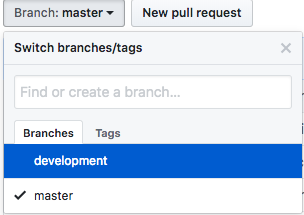
\includegraphics[width=0.5\textwidth]{images/branches}
    \caption{Push to New Branch}
\end{figure}

\end{subsubsection}
\end{subsection}

%%%%%%%%%%%%%%%%%%%%%%%%%%
% subsection: Github Workflow
%%%%%%%%%%%%%%%%%%%%%%%%%%
\begin{subsection}{Github Workflow}

Until now, we just talk about how to work alone. Group working is much more complex.
To help people working on Github, Github create a workflow called
\href{https://guides.github.com/introduction/flow/}{\underline{Github Flow}}.
It contains six steps:
\begin{enumerate}
    \item Create a branch
    \item Add commits
    \item Open a Pull request
    \item Discuss and review code
    \item Deploy
    \item Merge
\end{enumerate}

The core concept of this workflow is \textbf{Pull Request}. Pull request let
everybody participate in discussion and code review. Once the changes are approved,
the repository owner can choose th merge it into master branch.

\hypertarget{repo}{
\begin{figure}[ht]
    \centering
    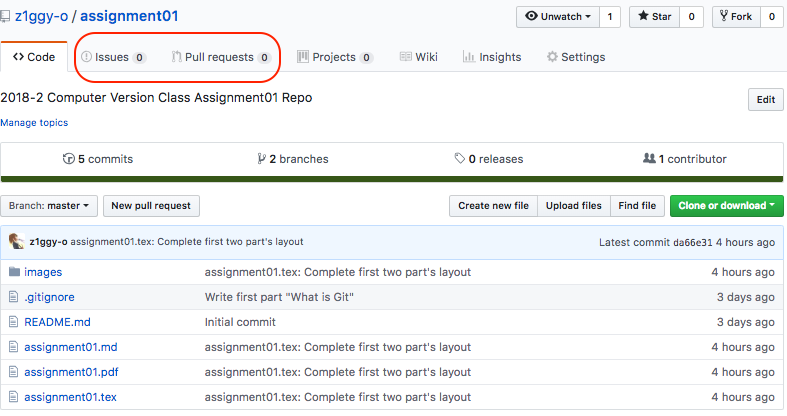
\includegraphics[width=1\textwidth]{images/github-repo}
    \caption{Github Repository}
\end{figure}
}

At our repository page's \textbf{Issue} and \textbf{Pull request} section,
people can discuss about the project or contribute to it.

There are many excellent open-source project on Github. Check those project's
pull request section can let you learn about them much faster.

\end{subsection}

\end{section}
\end{document}